\documentclass[a4paper,11pt]{article}
\input{/home/tof/Documents/Cozy/latex-include/preambule_lua.tex}
\newcommand{\showprof}{show them}  % comment this line if you don't want to see todo environment
\fancyhead[L]{Carte d'orientation - parcours}
\newdate{madate}{10}{09}{2020}
%\fancyhead[R]{\displaydate{madate}} %\today
%\fancyhead[R]{Seconde - SNT}
%\fancyhead[R]{Première - NSI}
\fancyhead[R]{Terminale - NSI}
\fancyfoot[L]{~\\Christophe Viroulaud}
\AtEndDocument{\label{lastpage}}
\fancyfoot[C]{\textbf{Page \thepage/\pageref{lastpage}}}
\fancyfoot[R]{\includegraphics[width=2cm,align=t]{/home/tof/Documents/Cozy/latex-include/cc.png}}
\usepackage{tikz}
\begin{document}
\begin{Form}
\begin{commentprof}
page 1 seule d'abord
\end{commentprof}
\section{Problématique}
Pour faire travailler ses élèves sur la carte de course d'orientation le professeur d'EPS organise plusieurs petits jeux. Il réalise par exemple plusieurs parcours d'une balise à une autre. Cependant selon les contraintes météorologiques certains chemins peuvent ne plus être praticables.
\begin{center}
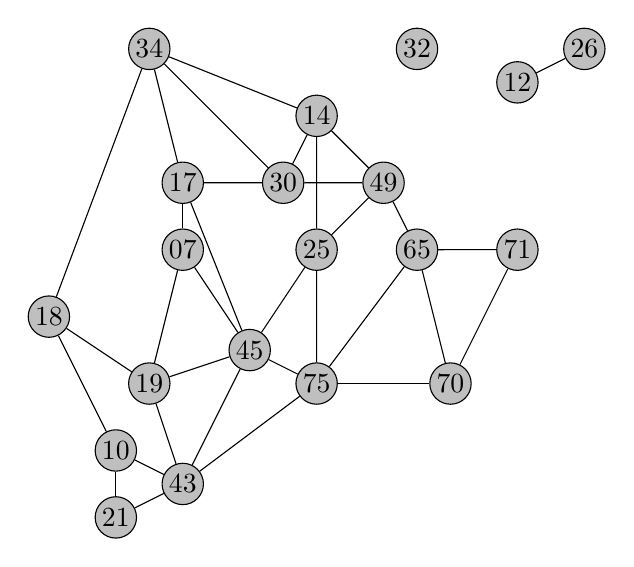
\begin{tikzpicture}[scale=0.85]
\node[draw,circle,fill=gray!50, inner sep=1.1] (21)at(0,0) {21};
\node[draw,circle,fill=gray!50, inner sep=1.1] (43)at(1,0.5) {43};
\node[draw,circle,fill=gray!50, inner sep=1.1] (10)at(0,1) {10};
\node[draw,circle,fill=gray!50, inner sep=1.1] (19)at(0.5,2) {19};
\node[draw,circle,fill=gray!50, inner sep=1.1] (45)at(2,2.5) {45};
\node[draw,circle,fill=gray!50, inner sep=1.1] (18)at(-1,3) {18};
\node[draw,circle,fill=gray!50, inner sep=1.1] (75)at(3,2) {75};
\node[draw,circle,fill=gray!50, inner sep=1.1] (70)at(5,2) {70};
\node[draw,circle,fill=gray!50, inner sep=1.1] (65)at(4.5,4) {65};
\node[draw,circle,fill=gray!50, inner sep=1.1] (71)at(6,4) {71};
\node[draw,circle,fill=gray!50, inner sep=1.1] (25)at(3,4) {25};
\node[draw,circle,fill=gray!50, inner sep=1.1] (07)at(1,4) {07};
\node[draw,circle,fill=gray!50, inner sep=1.1] (17)at(1,5) {17};
\node[draw,circle,fill=gray!50, inner sep=1.1] (30)at(2.5,5) {30};
\node[draw,circle,fill=gray!50, inner sep=1.1] (49)at(4,5) {49};
\node[draw,circle,fill=gray!50, inner sep=1.1] (14)at(3,6) {14};
\node[draw,circle,fill=gray!50, inner sep=1.1] (34)at(0.5,7) {34};
\node[draw,circle,fill=gray!50, inner sep=1.1] (32)at(4.5,7) {32};
\node[draw,circle,fill=gray!50, inner sep=1.1] (12)at(6,6.5) {12};
\node[draw,circle,fill=gray!50, inner sep=1.1] (26)at(7,7) {26};

\draw[-,>=latex] (75) -- (45);
\draw[-,>=latex] (75) -- (25);
\draw[-,>=latex] (75) -- (65);
\draw[-,>=latex] (75) -- (70);
\draw[-,>=latex] (75) -- (43);
\draw[-,>=latex] (45) -- (07);
\draw[-,>=latex] (45) -- (43);
\draw[-,>=latex] (45) -- (25);
\draw[-,>=latex] (45) -- (19);
\draw[-,>=latex] (45) -- (17);
\draw[-,>=latex] (25) -- (14);
%\draw[-,>=latex] (19) -- (10);
\draw[-,>=latex] (19) -- (18);
\draw[-,>=latex] (19) -- (07);
\draw[-,>=latex] (19) -- (43);
\draw[-,>=latex] (43) -- (10);
\draw[-,>=latex] (43) -- (21);
%\draw[-,>=latex] (43) -- (18);
\draw[-,>=latex] (10) -- (21);
\draw[-,>=latex] (10) -- (18);
\draw[-,>=latex] (34) -- (17);
\draw[-,>=latex] (70) -- (71);
\draw[-,>=latex] (70) -- (65);
\draw[-,>=latex] (49) -- (65);
\draw[-,>=latex] (49) -- (25);
\draw[-,>=latex] (49) -- (14);
\draw[-,>=latex] (49) -- (30);
%\draw[-,>=latex] (49) -- (32);
\draw[-,>=latex] (30) -- (14);
\draw[-,>=latex] (30) -- (34);
\draw[-,>=latex] (30) -- (17);
\draw[-,>=latex] (14) -- (34);
%\draw[-,>=latex] (14) -- (32);
%\draw[-,>=latex] (32) -- (12);
\draw[-,>=latex] (12) -- (26);
\draw[-,>=latex] (65) -- (71);
%\draw[-,>=latex] (71) -- (26);
\draw[-,>=latex] (18) -- (34);
\draw[-,>=latex] (07) -- (17);

\end{tikzpicture}
\captionof{figure}{Exemples de balises isolés}
\label{co}
\end{center}
\begin{center}
\shadowbox{\parbox{13cm}{\centering Peut-on construire des outils pour créer des parcours automatiquement et vérifier si toutes les balises sont atteignables?}}
\end{center}
\section{Connexité}
\subsection{Définition}
Une \textbf{chaîne} est une liste ordonnée de sommets du graphe dans laquelle chaque sommet est adjacent au suivant. 
Un graphe est \textbf{connexe} quand deux sommets quelconque peuvent être reliés par une chaîne.\\
Le graphe figure \ref{co} n'est pas connexe car la balise 32 n'est pas atteignable depuis un autre sommet.
\subsection{Parcours en profondeur (Depth First Search)}
\subsubsection{Méthodologie}
Pour vérifier la connexité d'un graphe une stratégie possible est celle que nous pourrions appliquer dans un labyrinthe: depuis notre point de départ nous suivons un chemin jusqu'à être bloqué puis nous faisons demi-tour jusqu'à la précédente intersection. Pour illustrer ce fonctionnement nous nous appuierons sur le graphe \ref{graphe0}.
\begin{commentprof}
algo pas précis ici volontairement: les élèves doivent détailler leur protocole dans l'activité 1. Notamment attention au cycle (et donc parcours en boucle).
\end{commentprof}
\begin{figure}[!h]
\centering
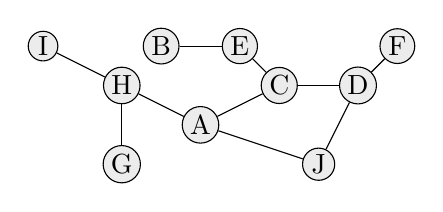
\begin{tikzpicture}[scale=0.5]
\node[draw,circle,fill=gray!15, inner sep=1.1] (A)at(0,0) {A};
\node[draw,circle,fill=gray!15, inner sep=1.1] (B)at(-1,2) {B};
\node[draw,circle,fill=gray!15, inner sep=1.1] (C)at(2,1) {C};
\node[draw,circle,fill=gray!15, inner sep=1.1] (D)at(4,1) {D};
\node[draw,circle,fill=gray!15, inner sep=1.1] (E)at(1,2) {E};
\node[draw,circle,fill=gray!15, inner sep=1.1] (F)at(5,2) {F};
\node[draw,circle,fill=gray!15, inner sep=1.1] (G)at(-2,-1) {G};
\node[draw,circle,fill=gray!15, inner sep=1.1] (H)at(-2,1) {H};
\node[draw,circle,fill=gray!15, inner sep=1.1] (I)at(-4,2) {I};
\node[draw,circle,fill=gray!15, inner sep=1.1] (J)at(3,-1) {J};
\draw[-,>=latex] (E) -- (B);
\draw[-,>=latex] (A) -- (C);
\draw[-,>=latex] (A) -- (H);
\draw[-,>=latex] (A) -- (J);
\draw[-,>=latex] (H) -- (I);
\draw[-,>=latex] (H) -- (G);
\draw[-,>=latex] (C) -- (E);
\draw[-,>=latex] (C) -- (D);
%\draw[-,>=latex] (C) -- (J);
\draw[-,>=latex] (D) -- (J);
\draw[-,>=latex] (D) -- (F);
\end{tikzpicture}
\captionof{figure}{Graphe étudié dans la suite}
\label{graphe0}
\end{figure}
\begin{activite}
Choisir un sommet et parcourir le graphe \guill{à la main} en détaillant le protocole appliqué.
\end{activite}
\subsubsection{Formalisation}
Détaillons l'algorithme du \textbf{parcours en profondeur}. Il est judicieux d'utiliser une pile pour stocker les sommets à visiter.
\begin{enumerate}
\item Initialisation: placer le sommet de départ dans la pile.
\item Tant qu'il reste des sommets dans la pile:
\begin{enumerate}
\item Dépiler le premier sommet de la pile.
\item S'il n'est pas marqué \emph{visité}:
\begin{itemize}
\item Le marquer \emph{visité}.
\item Placer chaque voisin de ce sommet dans la pile.
\end{itemize}
\end{enumerate}
\end{enumerate}
\begin{commentprof}
Il faut remarquer que nous pourrions n'ajouter que les voisins non encore visités. Ceci ne change rien au niveau de l'efficacité car il faut tout de même vérifier à chaque fois si le sommet est dans \emph{visités}.
\end{commentprof}
Appliquons l'algorithme sur le graphe \ref{graphe0}.

\bigskip
\begin{tabular}{>{\centering\arraybackslash}m{.4\textwidth} >{\centering\arraybackslash}m{.3\textwidth}
>{\centering\arraybackslash}m{.2\textwidth}}
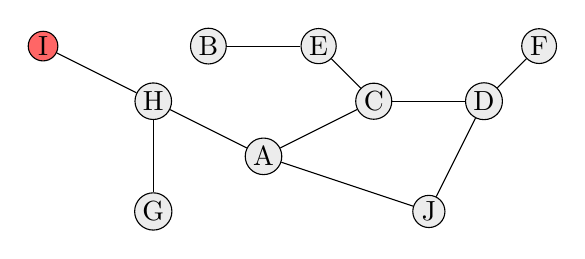
\begin{tikzpicture}[scale=0.7]
\node[draw,circle,fill=gray!15, inner sep=1.1] (A)at(0,0) {A};
\node[draw,circle,fill=gray!15, inner sep=1.1] (B)at(-1,2) {B};
\node[draw,circle,fill=gray!15, inner sep=1.1] (C)at(2,1) {C};
\node[draw,circle,fill=gray!15, inner sep=1.1] (D)at(4,1) {D};
\node[draw,circle,fill=gray!15, inner sep=1.1] (E)at(1,2) {E};
\node[draw,circle,fill=gray!15, inner sep=1.1] (F)at(5,2) {F};
\node[draw,circle,fill=gray!15, inner sep=1.1] (G)at(-2,-1) {G};
\node[draw,circle,fill=gray!15, inner sep=1.1] (H)at(-2,1) {H};
\node[draw,circle,fill=red!60, inner sep=1.1] (I)at(-4,2) {I};
\node[draw,circle,fill=gray!15, inner sep=1.1] (J)at(3,-1) {J};
\draw[-,>=latex] (E) -- (B);
\draw[-,>=latex] (A) -- (C);
\draw[-,>=latex] (A) -- (H);
\draw[-,>=latex] (A) -- (J);
\draw[-,>=latex] (H) -- (I);
\draw[-,>=latex] (H) -- (G);
\draw[-,>=latex] (C) -- (E);
\draw[-,>=latex] (C) -- (D);
%\draw[-,>=latex] (C) -- (J);
\draw[-,>=latex] (D) -- (J);
\draw[-,>=latex] (D) -- (F);
\end{tikzpicture} & Initialisation: 

le sommet I est empilé.

Sommets visités: $\emptyset$ &
Pile: \begin{tabular}{|c|}
\hline 
  \\ 
\hline 
  \\ 
\hline 
  \\  
\hline 
 I \\ 
\hline 
\end{tabular}  
\\
%ligne 2
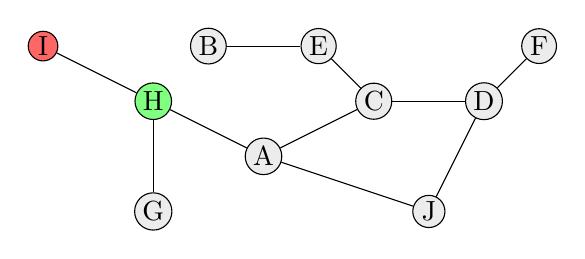
\begin{tikzpicture}[scale=0.7]
\node[draw,circle,fill=gray!15, inner sep=1.1] (A)at(0,0) {A};
\node[draw,circle,fill=gray!15, inner sep=1.1] (B)at(-1,2) {B};
\node[draw,circle,fill=gray!15, inner sep=1.1] (C)at(2,1) {C};
\node[draw,circle,fill=gray!15, inner sep=1.1] (D)at(4,1) {D};
\node[draw,circle,fill=gray!15, inner sep=1.1] (E)at(1,2) {E};
\node[draw,circle,fill=gray!15, inner sep=1.1] (F)at(5,2) {F};
\node[draw,circle,fill=gray!15, inner sep=1.1] (G)at(-2,-1) {G};
\node[draw,circle,fill=green!50, inner sep=1.1] (H)at(-2,1) {H};
\node[draw,circle,fill=red!60, inner sep=1.1] (I)at(-4,2) {I};
\node[draw,circle,fill=gray!15, inner sep=1.1] (J)at(3,-1) {J};
\draw[-,>=latex] (E) -- (B);
\draw[-,>=latex] (A) -- (C);
\draw[-,>=latex] (A) -- (H);
\draw[-,>=latex] (A) -- (J);
\draw[-,>=latex] (H) -- (I);
\draw[-,>=latex] (H) -- (G);
\draw[-,>=latex] (C) -- (E);
\draw[-,>=latex] (C) -- (D);
%\draw[-,>=latex] (C) -- (J);
\draw[-,>=latex] (D) -- (J);
\draw[-,>=latex] (D) -- (F);
\end{tikzpicture} & Le sommet I est dépilé et marqué \emph{visité}.

Les voisins sont empilés.

Sommets visités: I &
Pile: \begin{tabular}{|c|}
\hline 
  \\ 
\hline 
  \\ 
\hline 
  \\  
\hline 
 H \\ 
\hline 
\end{tabular}  
\\
%ligne 3
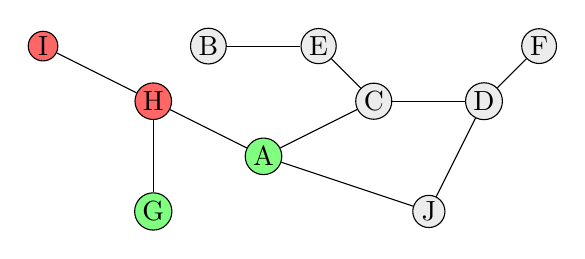
\begin{tikzpicture}[scale=0.7]
\node[draw,circle,fill=green!50, inner sep=1.1] (A)at(0,0) {A};
\node[draw,circle,fill=gray!15, inner sep=1.1] (B)at(-1,2) {B};
\node[draw,circle,fill=gray!15, inner sep=1.1] (C)at(2,1) {C};
\node[draw,circle,fill=gray!15, inner sep=1.1] (D)at(4,1) {D};
\node[draw,circle,fill=gray!15, inner sep=1.1] (E)at(1,2) {E};
\node[draw,circle,fill=gray!15, inner sep=1.1] (F)at(5,2) {F};
\node[draw,circle,fill=green!50, inner sep=1.1] (G)at(-2,-1) {G};
\node[draw,circle,fill=red!60, inner sep=1.1] (H)at(-2,1) {H};
\node[draw,circle,fill=red!60, inner sep=1.1] (I)at(-4,2) {I};
\node[draw,circle,fill=gray!15, inner sep=1.1] (J)at(3,-1) {J};
\draw[-,>=latex] (E) -- (B);
\draw[-,>=latex] (A) -- (C);
\draw[-,>=latex] (A) -- (H);
\draw[-,>=latex] (A) -- (J);
\draw[-,>=latex] (H) -- (I);
\draw[-,>=latex] (H) -- (G);
\draw[-,>=latex] (C) -- (E);
\draw[-,>=latex] (C) -- (D);
%\draw[-,>=latex] (C) -- (J);
\draw[-,>=latex] (D) -- (J);
\draw[-,>=latex] (D) -- (F);
\end{tikzpicture} & Le sommet H est dépilé et marqué visité.

Les voisins sont empilés.

Sommets visités: I, H &
Pile: \begin{tabular}{|c|}
\hline 
  \\ 
\hline 
 A \\ 
\hline 
 I \\  
\hline 
 G \\ 
\hline 
\end{tabular}  
\\
\end{tabular} 
\begin{activite}
\begin{enumerate}
\item Dérouler l'algorithme \guill{à la main} et vérifier sa correction.
\item À l'aide de la classe \emph{Graphe} du cours précédant, construire la représentation en mémoire du graphe \ref{graphe0}.
\item Dans la classe \emph{Graphe} ajouter la méthode \textbf{DFS(self, depart: str)$\;\rightarrow\;$list} qui renvoie la liste des sommets visités avec un parcours en profondeur, en partant de \emph{depart}.
\item Écrire la docstring de la méthode.
\end{enumerate}
\end{activite}
\subsubsection{Efficacité}
Chaque arête n'est examinée qu'une seule fois. La complexité de l'algorithme dépend donc directement du nombre d'arêtes du graphe.
\subsection{Vérifier la connexité}
Pour vérifier la connexité du graphe il suffit alors de vérifier si le nombre de sommets atteignables avec un parcours en profondeur correspond au nombre total de sommets du graphe.
\begin{activite}
Écrire la méthode \textbf{est\_connexe(self)$\;\rightarrow\;$bool} qui renvoie \emph{True} si le graphe est connexe.
\end{activite}
\section{Plus court chemin}
\subsection{Définition}
Le plus court chemin entre deux sommets correspond au nombre minimal d'arêtes pour relier ces deux sommets. Il n'y a pas encore ici de notion de distance entre deux balises sur la carte de CO.
\subsection{Parcours en largeur (Breadth First Search)}
\subsubsection{Méthodologie}
La stratégie consiste en la visite de tous les sommets à la distance 1 du sommet de départ, puis tous ceux à la distance 2 et ainsi de suite. Pour chaque sommet de rang \emph{n} nous pouvons accéder aux sommets de rang \emph{n+1}. Donc en partant du sommet de distance 0, nous pouvons accéder à tous les autres, s'ils sont connexes.
\begin{activite}
Choisir un sommet et parcourir le graphe \guill{à la main} en détaillant le protocole appliqué.
\end{activite}
\subsubsection{Formalisation}
Détaillons l'algorithme du \textbf{parcours en largeur}. Il est strictement identique au parcours en profondeur mais cette fois il est nécessaire d'utiliser une file pour stocker les sommets à visiter.
\begin{enumerate}
\item Initialisation: placer le sommet de départ dans la file.
\item Tant qu'il reste des sommets dans la file:
\begin{enumerate}
\item Défiler le premier sommet de la file.
\item S'il n'est pas marqué \emph{visité}:
\begin{itemize}
\item Le marquer \emph{visité}.
\item Placer chaque voisin de ce sommet dans la file.
\end{itemize}
\end{enumerate}
\end{enumerate}
Appliquons l'algorithme sur le graphe \ref{graphe0}.

\bigskip
\begin{tabular}{>{\centering\arraybackslash}m{.5\textwidth} >{\centering\arraybackslash}m{.5\textwidth}}
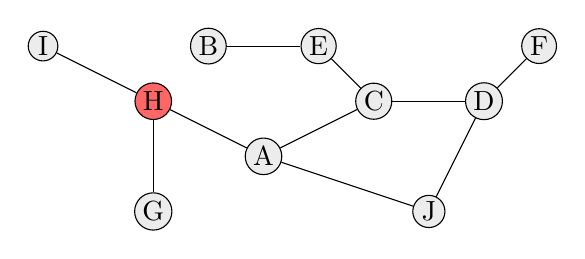
\begin{tikzpicture}[scale=0.7]
\node[draw,circle,fill=gray!15, inner sep=1.1] (A)at(0,0) {A};
\node[draw,circle,fill=gray!15, inner sep=1.1] (B)at(-1,2) {B};
\node[draw,circle,fill=gray!15, inner sep=1.1] (C)at(2,1) {C};
\node[draw,circle,fill=gray!15, inner sep=1.1] (D)at(4,1) {D};
\node[draw,circle,fill=gray!15, inner sep=1.1] (E)at(1,2) {E};
\node[draw,circle,fill=gray!15, inner sep=1.1] (F)at(5,2) {F};
\node[draw,circle,fill=gray!15, inner sep=1.1] (G)at(-2,-1) {G};
\node[draw,circle,fill=red!60, inner sep=1.1] (H)at(-2,1) {H};
\node[draw,circle,fill=gray!15, inner sep=1.1] (I)at(-4,2) {I};
\node[draw,circle,fill=gray!15, inner sep=1.1] (J)at(3,-1) {J};
\draw[-,>=latex] (E) -- (B);
\draw[-,>=latex] (A) -- (C);
\draw[-,>=latex] (A) -- (H);
\draw[-,>=latex] (A) -- (J);
\draw[-,>=latex] (H) -- (I);
\draw[-,>=latex] (H) -- (G);
\draw[-,>=latex] (C) -- (E);
\draw[-,>=latex] (C) -- (D);
%\draw[-,>=latex] (C) -- (J);
\draw[-,>=latex] (D) -- (J);
\draw[-,>=latex] (D) -- (F);
\end{tikzpicture} & Initialisation: 

le nœud H est enfilé

File: \begin{tabular}{|c|c|c|c|c|c|}
\hline 
H &  & & & & \\ 
\hline 
\end{tabular}  

Nœuds visités: $\emptyset$
\\
%ligne 2
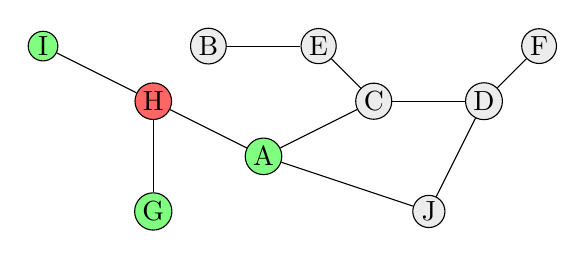
\begin{tikzpicture}[scale=0.7]
\node[draw,circle,fill=green!50, inner sep=1.1] (A)at(0,0) {A};
\node[draw,circle,fill=gray!15, inner sep=1.1] (B)at(-1,2) {B};
\node[draw,circle,fill=gray!15, inner sep=1.1] (C)at(2,1) {C};
\node[draw,circle,fill=gray!15, inner sep=1.1] (D)at(4,1) {D};
\node[draw,circle,fill=gray!15, inner sep=1.1] (E)at(1,2) {E};
\node[draw,circle,fill=gray!15, inner sep=1.1] (F)at(5,2) {F};
\node[draw,circle,fill=green!50, inner sep=1.1] (G)at(-2,-1) {G};
\node[draw,circle,fill=red!60, inner sep=1.1] (H)at(-2,1) {H};
\node[draw,circle,fill=green!50, inner sep=1.1] (I)at(-4,2) {I};
\node[draw,circle,fill=gray!15, inner sep=1.1] (J)at(3,-1) {J};
\draw[-,>=latex] (E) -- (B);
\draw[-,>=latex] (A) -- (C);
\draw[-,>=latex] (A) -- (H);
\draw[-,>=latex] (A) -- (J);
\draw[-,>=latex] (H) -- (I);
\draw[-,>=latex] (H) -- (G);
\draw[-,>=latex] (C) -- (E);
\draw[-,>=latex] (C) -- (D);
%\draw[-,>=latex] (C) -- (J);
\draw[-,>=latex] (D) -- (J);
\draw[-,>=latex] (D) -- (F);
\end{tikzpicture} & Le nœud H est défilé et marqué visité. 

Les voisins sont enfilés.

File: \begin{tabular}{|c|c|c|c|c|c|}
\hline 
A & G & I &  & & \\ 
\hline 
\end{tabular} 

Nœuds visités: H
\\
%ligne 3
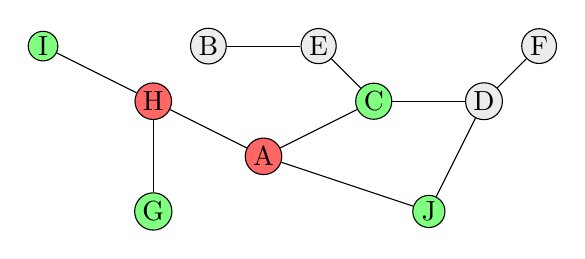
\begin{tikzpicture}[scale=0.7]
\node[draw,circle,fill=red!60, inner sep=1.1] (A)at(0,0) {A};
\node[draw,circle,fill=gray!15, inner sep=1.1] (B)at(-1,2) {B};
\node[draw,circle,fill=green!50, inner sep=1.1] (C)at(2,1) {C};
\node[draw,circle,fill=gray!15, inner sep=1.1] (D)at(4,1) {D};
\node[draw,circle,fill=gray!15, inner sep=1.1] (E)at(1,2) {E};
\node[draw,circle,fill=gray!15, inner sep=1.1] (F)at(5,2) {F};
\node[draw,circle,fill=green!50, inner sep=1.1] (G)at(-2,-1) {G};
\node[draw,circle,fill=red!60, inner sep=1.1] (H)at(-2,1) {H};
\node[draw,circle,fill=green!50, inner sep=1.1] (I)at(-4,2) {I};
\node[draw,circle,fill=green!50, inner sep=1.1] (J)at(3,-1) {J};
\draw[-,>=latex] (E) -- (B);
\draw[-,>=latex] (A) -- (C);
\draw[-,>=latex] (A) -- (H);
\draw[-,>=latex] (A) -- (J);
\draw[-,>=latex] (H) -- (I);
\draw[-,>=latex] (H) -- (G);
\draw[-,>=latex] (C) -- (E);
\draw[-,>=latex] (C) -- (D);
%\draw[-,>=latex] (C) -- (J);
\draw[-,>=latex] (D) -- (J);
\draw[-,>=latex] (D) -- (F);
\end{tikzpicture} & Le nœud A est défilé et marqué visité. 

Les voisins sont enfilés.

File: \begin{tabular}{|c|c|c|c|c|c|}
\hline 
G & I & C & J & H &\\ 
\hline 
\end{tabular} 

Nœuds visités: H, A
\end{tabular} 
\begin{activite}
\begin{enumerate}
\item Dérouler l'algorithme \guill{à la main} et vérifier sa correction.
\item Dans la classe \emph{Graphe} ajouter la méthode \textbf{BFS(self, depart: str)$\;\rightarrow\;$list} qui renvoie la liste des sommets visités avec un parcours en largeur, en partant de \emph{depart}.
\end{enumerate}
\end{activite}
\subsubsection{Efficacité}
Dans ce cas encore l'algorithme est très efficace car chaque arête n'est examinée qu'une seule fois. La complexité dépend du nombre d'arêtes du graphe.
\subsection{Trouver le plus court chemin}
Pour trouver le chemin le plus court entre deux sommets il faut adapter le parcours en largeur pour qu'il retienne la distance entre \emph{depart} et les autres sommets.
\begin{activite}
Écrire la méthode \textbf{plus\_court\_chemin(self, depart: str, arrivee: str)$\;\rightarrow\;$int}, adaptation de \emph{BFS} et qui renvoie le chemin entre \emph{depart} et \emph{arrivee}. Il sera nécessaire d'utiliser un dictionnaire \textbf{distances = \{depart: 0\}} qui retiendra les distances entre les sommets et \emph{depart}.
\end{activite}
\begin{commentprof}
BFS récursif est plus compliqué (moins naturel que DFS)
\end{commentprof}
\section{Application au parcours de CO}
\begin{activite}
\begin{enumerate}
\item Récupérer et modifier le fichier \emph{json} pour réaliser la situation de la figure \ref{co}.
\item Tester les méthodes précédemment réalisées.
\item Écrire la méthode \textbf{plus\_court\_chemin\_detail(self, depart: str, arrivee: str)$\;\rightarrow\;$list}, adaptation de \emph{plus\_court\_chemin} qui renvoie le chemin à parcourir pour atteindre \emph{arrivee} depuis \emph{depart}. Le processus se déroulera en deux étapes:
\begin{itemize}
\item déterminer le prédécesseur de chaque sommet,
\item puis reconstruire le chemin à partir des prédécesseurs. La méthode renverra \emph{None} si la balise n'est pas atteignable.
\end{itemize}
\end{enumerate}
Il est à noter que la méthode renvoie un chemin possible mais qu'il peut en exister d'autres.
\end{activite}
\end{Form}
\end{document}